\section{Tensore Energia-Impulso}
\subsection{Tensore energia-impulso}
In maniera analoga a quanto fatto in sezione \ref{sec:2.2}, ove, considerando una distribuzione di cariche, abbiamo definito la densità di carica e la densità di corrente, per poi unirle in un unico oggetto, al fine di trovare l'equazione di continuità. Considerando, nello stesso modo, una distribuzione di carica associamo, per ogni carica, un quadrimpulso: 
\begin{equation}
    P^\alpha_n=\left(\dfrac{E_n}{c}, \Vec{P}_n\right)=(\gamma m_nc,\gamma m_n \Vec{v}_n)
\end{equation}
A partire da questo possiamo definire la densità di energia-impulso come:
\begin{equation}
    T^{\alpha0}=c\sum_nP^\alpha_n\delta^3(\Vec{x}-\Vec{x}_n)
\end{equation}
e una densità di corrente di energia-impulso:
\begin{equation}
    T^{\alpha i}=\sum_nP^\alpha_n\delta^3(\Vec{x}-\Vec{x}_n)\dfrac{dx^i_n}{dt}(t)
\end{equation}
Ora, definiamo il \textit{tensore energia-impulso} come l'unione di questi oggetti:
\begin{equation}\phantomsection\label{eq:def_tens_E-I}
    T^{\alpha \beta}=\sum_nP^\alpha_n\delta^3(\Vec{x}-\Vec{x}_n)\dfrac{dx^\beta_n}{dt}(t)
\end{equation}
dimostriamo rapidamente che il tensore energia-impulso è simmetrico.
\begin{proof}
    Dalla definizione di quadrimpulso abbiamo che la componente spaziale si può scrivere:
    \begin{equation}
      \Vec{P}=\dfrac{E\Vec{v}}{c^2} \quad \text{ da cui segue} \quad P^\beta_n=\dfrac{E_n}{c^2}\dfrac{dx^\beta_n}{dt}
    \end{equation}
    sostituendola nella \eqref{eq:def_tens_E-I}, otteniamo:
    \begin{equation}
    T^{\alpha \beta}=\sum_nP^\alpha_n\delta^3(\Vec{x}-\Vec{x}_n)P^\beta_n\dfrac{c^2}{E_n}=c^2\sum_n\dfrac{P^\alpha_nP^\beta_n}{E_n}\delta^3(\Vec{x}-\Vec{x}_n)
\end{equation}
In tale forma risulta evidente la simmetria.\\
\end{proof}
Dalla \eqref{eq:def_tens_E-I} non è, tuttavia, evidente che sia un tensore, perciò dimostriamolo brevemente:
\begin{proof}
    Partiamo dalla definizione ed utiliziamo una delta di Dirac nel tempo:
    \begin{equation}
  \begin{aligned}
      T^{\alpha \beta}&=\sum_nP^\alpha_n\dfrac{dx^\beta_n}{dt}(t)\delta^3(\Vec{x}-\Vec{x}_n)=\int dt'\sum_nP^\alpha_n\dfrac{dx^\beta_n}{dt'}(t')\delta(t-t')\delta^3(\Vec{x}-\Vec{x}_n)\\
      &=c\int ds\sum_nP^\alpha_n\dfrac{dx^\beta_n}{ds}(s)\delta^4(x-x')
  \end{aligned}
\end{equation}
In tale forma risulta evidente la natura tensoriale dell'oggetto.\\
\end{proof}
Possiamo riconoscere negli elementi del tensore delle quantità importanti: la componente $T^{00}$ è la densità di energia, gli elementi $T^{i0}$ sono le densità delle componenti i-esime dell'impulso, mentre gli elementi $T^{0i}$ sono la densità del flusso di energia lungo $x^i$ ed, infine, gli elementi del tensore $3\times3$ $T^{ij}$ sono dette componenti del tensore degli sforzi di Maxwell\footnote{Nei casi che noi considereremo il tensore sarà sempre simmetrico, tuttavia ci sono casi in cui non lo è; ci sono delle procedure per simmetrizzarlo che consistono nell'aggiunta di altri tensori. La ragione per cui si ricercano tensori energia-impulso simmetrici è che in relatività generale, nelle equazioni di campo di Einstein, il membro sinistro risulta simmetrico e il membro destro è il tensore energia-impulso (la sorgente).}.

Vogliamo, ora, determinare un'equazione di continuità. Per farlo consideriamo la divergenza di $T^{\alpha \beta}$ e utilizziamo la proprietà secondo cui se una funzione ha una dipendenza del tipo $F(x-y)$, allora vale l'identità $\dfrac{\partial F}{\partial x}=-\dfrac{\partial F}{\partial y}$:
  \begin{equation}
  \begin{aligned}
      \dfrac{\partial}{\partial x^i}T^{\alpha i}&=\sum_nP^\alpha_n(t)\dfrac{\partial x^i_n}{\partial t} \dfrac{\partial }{\partial x^i}\delta^3(\Vec{x}-\Vec{x}_n)=-\sum_nP^\alpha_n(t)\dfrac{\partial x^i_n}{\partial t} \dfrac{\partial}{\partial x^i_n}\delta^3(\Vec{x}-\Vec{x}_n)\\
      &=-\sum_nP^\alpha_n(t)\dfrac{\partial }{\partial t} \delta^3(\Vec{x}-\Vec{x}_n)=-\dfrac{1}{c}\dfrac{\partial T^{\alpha 0}}{\partial t}+\sum_n\dfrac{dP^\alpha_n}{dt}(t)\delta^3(\Vec{x}-\Vec{x}_n)
  \end{aligned}
\end{equation}
ove nell'ultimo passaggio, a causa della dipendenza del quadrimpulso dal tempo, consideriamo la derivata della delta come la sottrazione tra la derivata del prodotto meno la derivata rispetto a $P^\alpha_n$.
Riscriviamo l'ultima relazione come:
 \begin{equation}
 \dfrac{\partial}{\partial x^i}T^{\alpha i}+\dfrac{1}{c}\dfrac{\partial T^{\alpha 0}}{\partial t}=\sum_n\dfrac{dP^\alpha_n}{dt}(t)\delta^3(\Vec{x}-\Vec{x}_n)
\end{equation}
possiamo riscrivere l'equazione considerando la quadridivergenza
\begin{equation}\phantomsection\label{eq:Quaddiv_tens_E-I}
 \dfrac{d}{dx^\beta}T^{\alpha \beta}=\sum_n\delta^3(\Vec{x}-\Vec{x}_n)\dfrac{dP^\alpha_n}{dt}(t)
\end{equation}
Nel caso di particelle libere avremo che:
\begin{equation}
    \dfrac{dP^\alpha_n}{dt}=0 \implies\dfrac{d}{dx^\beta}T^{\alpha \beta}=0
\end{equation}
quindi, dalla definizione del tensore energia-impulso avremo che:
\begin{equation}
    P^\alpha=\int d^3x \quad T^{\alpha0}
\end{equation}
derivando nel tempo
\begin{equation}
 \dfrac{1}{c}  \dfrac{dP^\alpha}{dt}=\int d^3x\quad \dfrac{1}{c} \partial_t T^{\alpha0}=-\int d^3x \quad\partial_i T^{\alpha i}=-\int_\Sigma d\Sigma\quad T^{\alpha i}=0
\end{equation}
ove nell'ultimo passaggio si è utilizzato il teorema di Gauss. Concludiamo che in questo caso particolare il quadrimpulso è conservato, tuttavia dalla \eqref{eq:Quaddiv_tens_E-I} in generale sembrerebbe di no. La questione risulta essere problematica. Per  risolverla bisogna considerare gli scambi tra particelle e campo, sarà il quadrimpulso totale a doversi conservare.
\subsection{Particelle cariche in un campo elettromagnetico}
Sulla base di quanto appreso nel precedente capitolo, applichiamo le nuove conoscenze al caso di particelle immerse in un campo elettromagnetico. Ricordiamo, dallo studio della dinamica in sezione \ref{sec:2.1}, che la forza di Lorentz è:
\begin{equation}
     \dfrac{dP^\alpha}{ds}=\dfrac{e_n}{c}F^{\alpha\beta}u_\beta
\end{equation}
questa relazione considera una sola carica, ovviamente per rendere il conto generale bisogna considerare una sommatoria nelle n.
Possiamo riscrivere la relazione precedente in funzione di $dt$ e attraverso la matrice metrica possiamo alzare ed abbassare indici
\begin{equation}
\begin{gathered}
     \dfrac{dP^\alpha}{dt}\dfrac{dt}{ds}=\dfrac{e_n}{c}F^\alpha_\beta u^\beta=\dfrac{e_n}{c}F^\alpha_\beta \dfrac{dx_n^\beta}{dt}\dfrac{dt}{ds}\\
     \implies\dfrac{dP^\alpha}{dt}=\dfrac{e_n}{c}F^\alpha_\beta \dfrac{dx_n^\beta}{dt}
\end{gathered}
\end{equation}
sostituendo nella \eqref{eq:Quaddiv_tens_E-I} otteniamo il tensore energia impulso del sistema di particelle:
\begin{equation}\phantomsection\label{eq:tens_par}
 \dfrac{d}{dx^\beta}T^{\alpha \beta}_{par}=\sum_n\dfrac{e_n}{c}F^\alpha_\gamma \dfrac{dx_n^\gamma}{dt}\delta^3(\Vec{x}-\Vec{x}_n)=\dfrac{1}{c}F^\alpha_\gamma j^\gamma
\end{equation}
quindi il quadrimpulso non si conserva, ma ricordiamo, questo è il quadrimpulso delle particelle. Quello che il buon senso fisico suggerisce è che sia il quadrimpulso totale, comprendente anche del quadrimpulso del campo a conservarsi $P^\alpha_T=P^\alpha_{par}+P^\alpha_{cam}$, ossia $\dfrac{dP^\alpha_T}{dt}=0$.

Possiamo introdurre il tensore energia-impulso del campo elettromagnetico:
\begin{equation}
 T^{\alpha \beta}_{cam}=-\dfrac{1}{4\pi}\left(F^\alpha_\gamma F^{\beta\gamma}- \dfrac{1}{4}\eta^{\alpha\beta}F_{\gamma\delta} F^{\gamma\delta} \right)
\end{equation}
notiamo che le componenti 
\begin{equation}
    \begin{gathered}
        T^{00}_{cam}=\dfrac{1}{8\pi}(E^2+B^2)\\
        T^{0i}_{cam}=\dfrac{1}{4\pi}(\Vec{E}\times\Vec{B})_i
    \end{gathered}
\end{equation}
sono, rispettivamente, la densità di energia del campo elettromagnetico e il vettore di Poynting. 

 Come già dimostrato in generale, il tensore è simmetrico $T^{\alpha \beta}_{cam}=T^{\beta \alpha}_{cam}$, un'altra proprietà interessante è che ha traccia nulla, per mostrarlo abbassiamo un indice e contraiamolo:
\begin{equation}
 T\indices{_{cam}^\alpha_\alpha}=-\dfrac{1}{4\pi}\left(F^\alpha_\gamma F^\gamma_\alpha- \dfrac{1}{4}\delta^\alpha_\alpha F_{\gamma\delta} F^{\gamma\delta} \right)=-\dfrac{1}{4\pi}\left(F^{\alpha\gamma} F_{\gamma\alpha}- F_{\gamma\delta} F^{\gamma\delta} \right)=0
\end{equation}
ove $\delta^\alpha_\gamma=4$ poiché siamo in uno spazio quadridimensionale, in altre dimensioni non è detto che la traccia sia nulla. Ora calcoliamoci la quadridivergenza:
\begin{equation}
\begin{aligned}
\dfrac{d}{dx^\beta}T^{\alpha\beta}_{cam}&=-\dfrac{1}{4\pi}\left[\partial_\beta(F^\alpha_\gamma)F^{\beta\gamma}+F^\alpha_\gamma\partial_\beta(F^{\beta\gamma})- \dfrac{1}{4}\partial_\beta(\eta^{\alpha\beta}F_{\gamma\delta} F^{\gamma\delta}) \right]\\
&=-\dfrac{1}{4\pi}\left[\partial_\beta(F^\alpha_\gamma)F^{\beta\gamma}+F^\alpha_\gamma\partial_\beta(F^{\beta\gamma})- \dfrac{1}{4}\partial^\alpha(F_{\gamma\delta} F^{\gamma\delta}) \right]\\
&=-\dfrac{1}{4\pi}\left[\partial^\beta(F^{\alpha\gamma})F_{\beta\gamma}+F^\alpha_\gamma\partial_\beta(F^{\beta\gamma})- \dfrac{1}{4}\partial^\alpha(F_{\gamma\delta}) F^{\gamma\delta}- \dfrac{1}{4}\partial^\alpha(F^{\gamma\delta}) F_{\gamma\delta} \right]\\
&\text{Riconosciamo nel secondo termine, l'equazione di Maxwell non omogenea \eqref{eq:eq_non_omo}:}
\\
\dfrac{d}{dx^\beta}T^{\alpha\beta}_{cam}&=-\dfrac{1}{4\pi}\left[\partial^\beta(F^{\alpha\gamma})F_{\beta\gamma}+F^\alpha_\gamma\dfrac{4\pi}{c}j^\gamma- \dfrac{1}{4}\partial^\alpha(F^{\gamma\delta}) F_{\gamma\delta} - \dfrac{1}{4}\partial^\alpha(F^{\gamma\delta}) F_{\gamma\delta}  \right]\\
&=-\dfrac{1}{c}F^\alpha_\gamma j^\gamma-\dfrac{1}{4\pi}\left[\partial^\beta(F^{\alpha\gamma})F_{\beta\gamma}- \dfrac{1}{2}\partial^\alpha(F^{\gamma\delta}) F_{\gamma\delta}   \right]\\
&\text{nell'ultimo termine $\delta$ è un indice di sommatoria, possiamo ribattezzarlo $\beta$}\\
\dfrac{d}{dx^\beta}T^{\alpha\beta}_{cam}&=-\dfrac{1}{c}F^\alpha_\gamma j^\gamma-\dfrac{1}{4\pi}\left[\partial^\beta(F^{\alpha\gamma})F_{\beta\gamma}- \dfrac{1}{2}\partial^\alpha(F^{\gamma\beta}) F_{\gamma\beta}   \right]
\end{aligned}
\end{equation}
studiamo i termini rimasti dentro la quadra, al fine di dimostrare che è nulla. Partiamo dal primo termine:
\begin{equation}
\begin{aligned}
\partial^\beta(F^{\alpha\gamma})&=\dfrac{2}{2}\partial^\beta(F^{\alpha\gamma})+\dfrac{1}{2}\partial^\gamma(F^{\alpha\beta})-\dfrac{1}{2}\partial^\gamma(F^{\alpha\beta})\\
&=\dfrac{1}{2}(\partial^\beta F^{\alpha\gamma}+\partial^\gamma F^{\alpha\beta})+\dfrac{1}{2}(\partial^\beta F^{\alpha\gamma}-\partial^\gamma F^{\alpha\beta})
\end{aligned}
\end{equation}
notiamo che il primo termine è simmetrico per lo scambio $\beta\leftrightarrow\gamma$ mentre il secondo è antisimmetrico, quindi moltiplicandolo per il tensore elettromagnetico, il quale è antisimmetrico, sopravvive solo il termine antisimmetrico ed otteniamo:
\begin{equation}
\begin{aligned}
\partial^\beta(F^{\alpha\gamma})F_{\beta\gamma}&=+\dfrac{1}{2}(\partial^\beta F^{\alpha\gamma}-\partial^\gamma F^{\alpha\beta})F_{\beta\gamma}
\end{aligned}
\end{equation}
sostituendo quest'ultimo risultato nella quadra troviamo:
\begin{equation}
\begin{aligned}
\dfrac{d}{dx^\beta}T^{\alpha\beta}_{cam}&=-\dfrac{1}{c}F^\alpha_\gamma j^\gamma-\dfrac{1}{4\pi}\left[\dfrac{1}{2}(\partial^\beta F^{\alpha\gamma}-\partial^\gamma F^{\alpha\beta})F_{\beta\gamma}-\dfrac{1}{2}\partial^\alpha(F^{\gamma\beta}) F_{\gamma\beta}   \right]\\
&=-\dfrac{1}{c}F^\alpha_\gamma j^\gamma-\dfrac{1}{4\pi}\left[\dfrac{1}{2}(\partial^\beta F^{\alpha\gamma}-\partial^\gamma F^{\alpha\beta})F_{\beta\gamma}+\dfrac{1}{2}\partial^\alpha(F^{\gamma\beta}) F_{\beta\gamma}   \right]\\
&=-\dfrac{1}{c}F^\alpha_\gamma j^\gamma-\dfrac{1}{8\pi}\left[\partial^\beta F^{\alpha\gamma}-\partial^\gamma F^{\alpha\beta} +\partial^\alpha F^{\gamma\beta}   \right]F_{\beta\gamma}\\
&=-\dfrac{1}{c}F^\alpha_\gamma j^\gamma-\dfrac{1}{8\pi}\left[\partial^\beta F^{\alpha\gamma}+\partial^\gamma F^{\beta\alpha} +\partial^\alpha F^{\gamma\beta}   \right]F_{\beta\gamma}\\
\end{aligned}
\end{equation}
dall'equazione \eqref{eq:omo_no_duale} otteniamo
\begin{equation}\phantomsection\label{eq:tens_camp}
\dfrac{d}{dx^\beta}T^{\alpha\beta}_{cam}=-\dfrac{1}{c}F^\alpha_\gamma j^\gamma
\end{equation}

A questo punto possiamo definire il tensore energia-impulso totale e sostituendo le \eqref{eq:tens_par} \eqref{eq:tens_camp}:
\begin{equation}\phantomsection\label{eq:tens_cont}
T^{\alpha\beta}_T=T^{\alpha\beta}_{par}+T^{\alpha\beta}_{cam} \implies\dfrac{d}{dx^\beta}T^{\alpha\beta}_T=\dfrac{d}{dx^\beta}T^{\alpha\beta}_{par}+\dfrac{d}{dx^\beta}T^{\alpha\beta}_{cam}=0
\end{equation}
da cui segue che 
\begin{equation}
P^{\alpha}_T=P^{\alpha}_{par}+P^{\alpha}_{cam}=\int d^3x\quad T^{\alpha0}_{par}+T^{\alpha0}_{cam}
\end{equation}
si conserva.

\subsection{Fluidi perfetti}

Il tensore energia-impulso è particolarmente usato nei modelli della fisica che si basano sui, così detti, \textit{fluidi perfetti}. Moltissimi sistemi fisici possono essere descritti, con opportune approssimazioni, come fluidi. I fluidi perfetti sono modellizzazioni ideali di fluidi con viscosità nulla e senza capacità di condurre calore\footnote{Ciò significa che il flusso del fluido è legato solo al moto delle particelle che lo costituiscono.}. Consideriamo un fluido in movimento, in particolare definiamo un sistema di riferimento comovente con il fluido, si veda Fig.\ref{fig:fluido}. 
\begin{figure}[H]
    \centering
    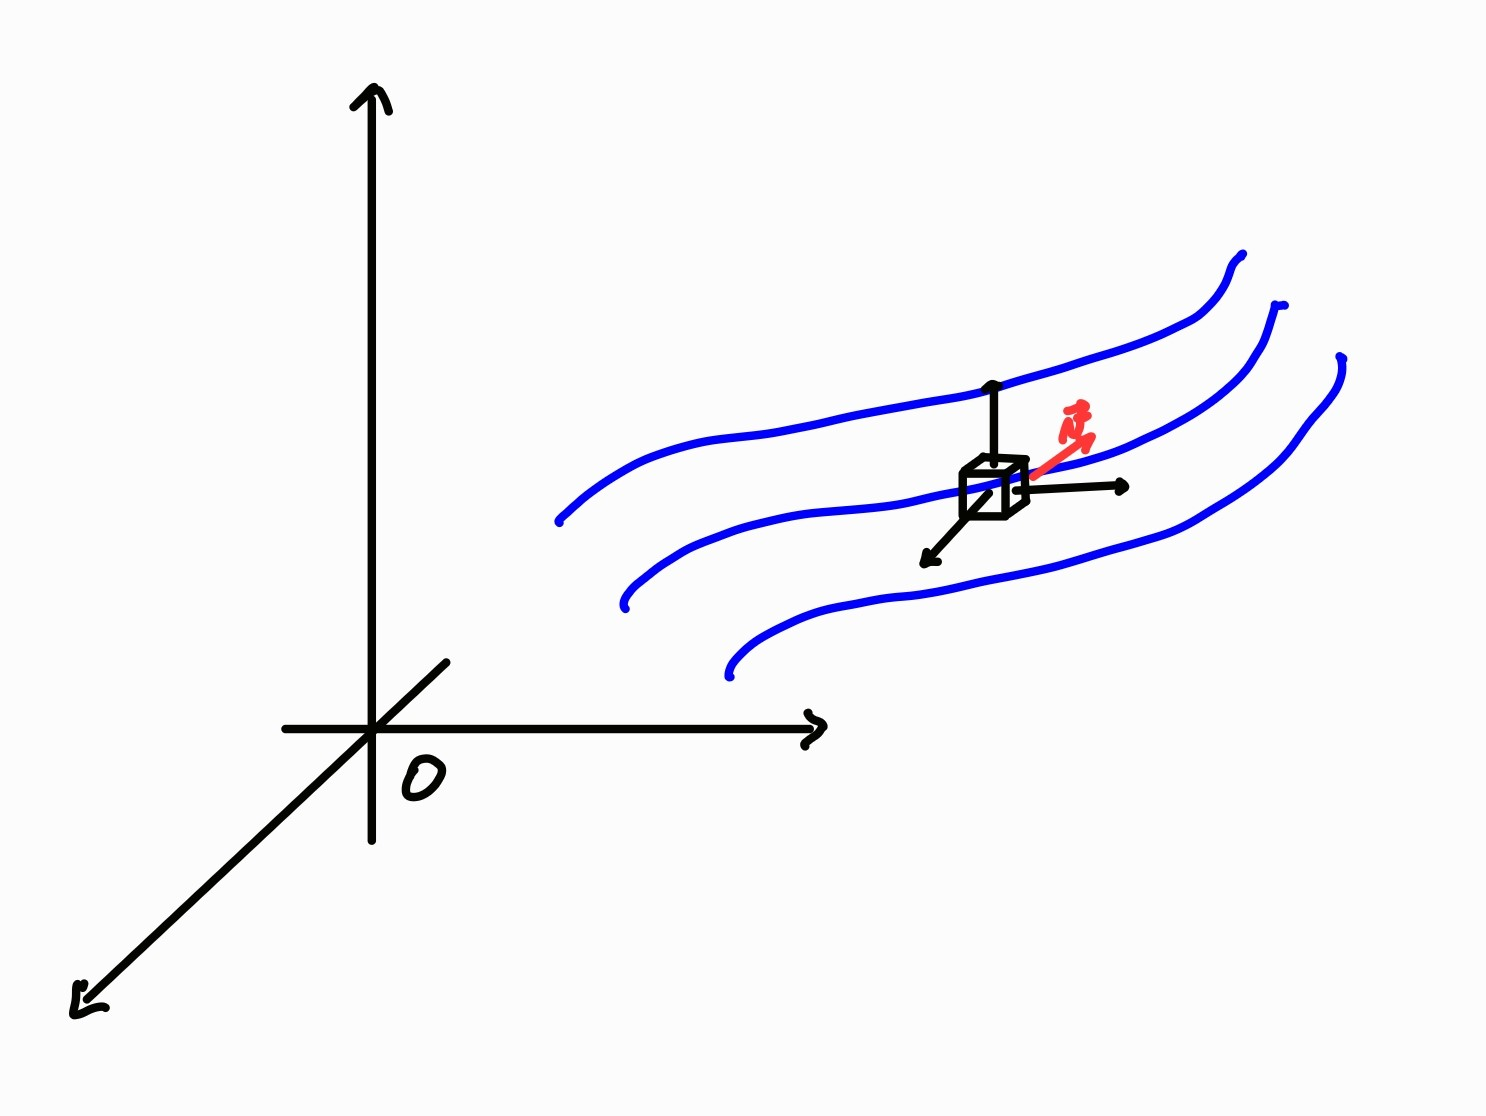
\includegraphics[width=0.31\textwidth]{Immagini/Fluido.jpg}
    \caption{Fluido perfetto in moto.}
    \label{fig:fluido}
\end{figure}
In tale sistema il tensore energia-impulso associato al fluido deve essere isotropo ed  assume la semplice forma:
\begin{equation}
\Tilde{T}\indices{^\gamma_\beta}=
\begin{pmatrix}
  \rho & 0 & 0 & 0  \\
  0 & p & 0 & 0  \\
  0 & 0 & p & 0   \\
  0 & 0 & 0 & p
\end{pmatrix}
\end{equation}
ove $\rho$ è la densità di energia e $p$ la pressione nel sistema comovente\footnote{Osserviamo che ai sistemi è associabile un'equazione di stato. Un esempio semplice si ha quando l'equazione di stato è  $p=0$, anche detta della polvere.}. Mentre in un sistema fisso, per esempio di un laboratorio, il sistema comovente avrà una certa velocità $\Vec{v}$, in generale, variabile localmente. Ci aspettiamo che la trasformazione che leghi i tensori energia-impulso sia una trasformazione di Lorentz:
\begin{equation}
T\indices{^{\alpha\beta}}=\Lambda\indices{^\alpha_\mu}(-\Vec{v})\Lambda\indices{^\beta_\nu}(-\Vec{v})\Tilde{T}\indices{^{\mu\nu}}
\end{equation}
ricordiamo che, in generale, la matrice di trasformazione ha le componenti \eqref{eq:generic_elem_tras}. 

Determiniamo le componenti del tensore energia-impulso nel sistema generico:
\begin{equation}
\begin{aligned}
    T^{00}&=\Lambda\indices{^0_\mu}\Lambda\indices{^0_\nu}\Tilde{T}\indices{^{\mu\nu}}=\Lambda\indices{^0_0}\Lambda\indices{^0_0}\Tilde{T}\indices{^{00}}+\Lambda\indices{^0_i}\Lambda\indices{^0_j}\Tilde{T}\indices{^{ij}}=\gamma^2\rho+\gamma^2\beta_i\beta_jp\delta_{ij}\\
    &=\gamma^2(\rho+\beta^2p)=\gamma^2\rho+\gamma^2\beta^2p=\gamma^2\rho+\dfrac{\beta^2}{1-\beta^2}p=\gamma^2\rho+(\gamma^2-1)p=\gamma^2(\rho+p)-p
    \end{aligned}
\end{equation}
consideriamo ora le componenti:
\begin{equation}
\begin{aligned}
   T^{i0}= T^{0i}&=\Lambda\indices{^0_\mu}\Lambda\indices{^i_\nu}\Tilde{T}\indices{^{\mu\nu}}=\Lambda\indices{^0_0}\Lambda\indices{^i_0}\Tilde{T}\indices{^{i0}}+\Lambda\indices{^0_j}\Lambda\indices{^i_k}\Tilde{T}\indices{^{jk}}=\gamma^2\beta_i\rho+\beta_j\gamma\left[\delta_{ik}+(\gamma-1)\dfrac{\beta_i\beta_k}{\beta^2}\right]p\delta_{jk}\\
   &=\gamma^2\beta_i\rho+\beta_j\gamma\left[\delta_{ij}+(\gamma-1)\dfrac{\beta_i\beta_j}{\beta^2}\right]p=\gamma^2\beta_i\rho+\beta_i\gamma p+\gamma(\gamma-1)\dfrac{\beta^2\beta_i}{\beta^2}p\\
   &=\gamma^2\beta_i\rho+\beta_i\gamma p+(\gamma^2-\gamma)\beta_ip=\gamma^2\beta_i(\rho+p)
    \end{aligned}
\end{equation}
infine rimane:
\begin{equation}
\begin{aligned}
   T^{ij}&=\Lambda\indices{^i_\mu}\Lambda\indices{^j_\nu}\Tilde{T}\indices{^{\mu\nu}}=\Lambda\indices{^i_0}\Lambda\indices{^j_0}\Tilde{T}\indices{^{i0}}+\Lambda\indices{^i_k}\Lambda\indices{^j_l}\Tilde{T}\indices{^{kl}}\\
   &=\gamma^2\beta_i\beta_j\rho+\left[\delta_{ik}+(\gamma-1)\dfrac{\beta_i\beta_k}{\beta^2}\right]\left[\delta_{jl}+(\gamma-1)\dfrac{\beta_j\beta_l}{\beta^2}\right]p\delta_{kl}\\
   &=\gamma^2\beta_i\beta_j\rho+\left[\delta_{ij}+(\gamma-1)\dfrac{\beta_i\beta_j}{\beta^2}+(\gamma-1)\dfrac{\beta_i\beta_j}{\beta^2}+(\gamma-1)^2\dfrac{(\beta_i\beta_j)(\beta_k\beta_k)}{\beta^2\beta^2}\right]p\\
   &=\gamma^2\beta_i\beta_j\rho+\left\{\delta_{ij}+\dfrac{\beta_i\beta_j}{\beta^2}[2(\gamma-1)+(\gamma-1)^2]\right\}p\\
   &=\gamma^2\beta_i\beta_j\rho+\left\{\delta_{ij}+\dfrac{\beta_i\beta_j}{\beta^2}[2(\gamma-1)+(\gamma^2-2\gamma+1)]\right\}p\\
   &=\gamma^2\beta_i\beta_j\rho+\left[\delta_{ij}+\dfrac{\beta_i\beta_j}{\beta^2}(\gamma^2-1)\right]p=\gamma^2\beta_i\beta_j\rho+\left[\delta_{ij}+\dfrac{\beta_i\beta_j}{\beta^2}(\dfrac{1}{1-\beta^2}-1)\right]p\\
   &=\gamma^2\beta_i\beta_j\rho+\left[\delta_{ij}+\dfrac{\beta_i\beta_j}{\beta^2}\left(\dfrac{\beta^2}{1-\beta^2}\right)\right]p=\gamma^2\beta_i\beta_j\rho+\left[\delta_{ij}+\dfrac{\beta_i\beta_j}{1-\beta^2}\right]p\\
   &=\gamma^2\beta_i\beta_j\rho+\delta_{ij}p+\gamma^2\beta_i\beta_jp=\gamma^2\beta_i\beta_j(\rho+p)+\delta_{ij}p
   \end{aligned}
\end{equation}
A partire da queste tre relazioni vogliamo scrivere una sola equazione covariante. Per farlo, consideriamo la quadrivelocità $u^\mu=(\gamma,\gamma\Vec{\beta})$ e riscriviamo tutte le relazioni precedenti:
\begin{equation}
     T^{00}=\gamma^2(\rho+p)-p=(\rho+p)u^0u^0-\eta^{00}p
\end{equation}
\begin{equation}
     T^{i0}=\gamma^2\beta_i(\rho+p)=(\rho+p)u^0u^i
\end{equation}
\begin{equation}
    T^{ij}=\gamma^2\beta_i\beta_j(\rho+p)+\delta_{ij}p=(\rho+p)u^iu^j-\eta^{ij}p
\end{equation}
concludiamo che la forma covariante compatta è:\begin{equation}\phantomsection\label{eq:tensore_fluidi}
    T^{\mu\nu}=(\rho+p)u^\mu u^\nu -\eta^{\mu\nu}p
\end{equation}
Consideriamo, ora, che il sistema sia isolato e quindi:
\begin{equation}
\begin{gathered}
    \dfrac{dT^{\alpha\beta}}{dx^\beta}=0 \\ 
    \dfrac{d}{dx^\beta}[(\rho+p)u^\alpha u^\beta]-\dfrac{d}{dx^\beta}[\eta^{\alpha\beta}p]=0\\
    \dfrac{d}{dx^\beta}[(\rho+p)u^\alpha u^\beta]-\dfrac{dp}{dx_\alpha}=0
\end{gathered}
\end{equation}
ove nell'ultimo passaggio si è utilizzata la proprietà di innalzamento di indice per la derivata; la relazione è ovviamente vettoriale, dunque consideriamo componente per componente. 

Fissiamo $\alpha=0$ e notiamo che $u^j=u^0\beta^j$:
\begin{equation}\phantomsection\label{eq:alfa_0}
\begin{gathered}
   \dfrac{d}{dx^\beta}[(\rho+p)u^0 u^\beta]-\dfrac{dp}{dx_0}=0\\
  \dfrac{1}{c} \dfrac{d}{dt}[(\rho+p)u^0 u^0]+ \dfrac{d}{dx^j}[(\rho+p)u^0 u^j]-\dfrac{1}{c}\dfrac{dp}{dt}=0\\
   \dfrac{1}{c}\dfrac{d}{dt}[(\rho+p)(u^0)^2]+ \dfrac{d}{dx^j}[(\rho+p)(u^0)^2 \frac{v^j}{c}]-\dfrac{1}{c}\dfrac{dp}{dt}=0
\end{gathered}
\end{equation}
ora consideriamo $\alpha=i$ (ossia le coordinate spaziali):
\begin{equation}
\begin{gathered}
   \dfrac{d}{dx^\beta}[(\rho+p)u^i u^\beta]-\dfrac{dp}{dx_i}=0\\
   \dfrac{d}{dx^0}[(\rho+p)u^i u^0]+\dfrac{d}{dx^j}[(\rho+p)u^i u^j]-\dfrac{dp}{dx_i}=0\\
    \dfrac{1}{c}\dfrac{d}{dt}[(\rho+p)(u^0)^2\frac{v^i}{c}]+\dfrac{d}{dx^j}[(\rho+p)(u^0)^2\frac{v^i}{c}\frac{v^j}{c}]+\dfrac{dp}{dx^i}=0\\
\end{gathered}
\end{equation}

    \begin{equation*}
          \dfrac{1}{c^2}\dfrac{dv^i}{dt}[(\rho+p)(u^0)^2]+\dfrac{v^i}{c^2}\dfrac{d}{dt}[(\rho+p)(u^0)^2]+\dfrac{1}{c^2}\dfrac{dv^i}{dx^j}[(\rho+p)(u^0)^2v^j]+\dfrac{v^i}{c^2}\dfrac{d}{dx^j}[(\rho+p)(u^0)^2v^j]+\dfrac{dp}{dx^i}=0\\
    \end{equation*}
      

usando la \eqref{eq:alfa_0} otteniamo $ \dfrac{1}{c}\dfrac{d}{dt}[(\rho+p)(u^0)^2]=+\dfrac{1}{c}\dfrac{dp}{dt}- \dfrac{1}{c}\dfrac{d}{dx^j}[(\rho+p)(u^0)^2 v^j]$, che sostituendola nella precedente:
\begin{equation*}
\begin{aligned}
    \dfrac{1}{c^2}\dfrac{dv^i}{dt}[(\rho+p)(u^0)^2]&+\dfrac{v^i}{c}\left\{+\dfrac{1}{c}\dfrac{dp}{dt}- \dfrac{1}{c}\dfrac{d}{dx^j}[(\rho+p)(u^0)^2 v^j]\right\}\\
    &+\dfrac{1}{c^2}\dfrac{dv^i}{dx^j}[(\rho+p)(u^0)^2v^j]+\dfrac{v^i}{c^2}\dfrac{d}{dx^j}[(\rho+p)(u^0)^2v^j]+\dfrac{dp}{dx^i}=0
\end{aligned}
\end{equation*}
\begin{equation}
\begin{aligned}
        \dfrac{1}{c^2}\dfrac{dv^i}{dt}[(\rho+p)(u^0)^2]&+\dfrac{v^i}{c^2}\dfrac{dp}{dt}-\dfrac{v^j}{c^2} \dfrac{d}{dx^j}[(\rho+p)(u^0)^2 v^j]\\
    &+\dfrac{1}{c^2}\dfrac{dv^i}{dx^j}[(\rho+p)(u^0)^2v^j]+\dfrac{v^i}{c^2}\dfrac{d}{dx^j}[(\rho+p)(u^0)^2v^j]+\dfrac{dp}{dx^i}=0
\end{aligned}
\end{equation}
\begin{equation*}
        \dfrac{1}{c^2}\dfrac{dv^i}{dt}[(\rho+p)(u^0)^2]+\dfrac{v^i}{c^2}\dfrac{dp}{dt}+\dfrac{1}{c^2}\dfrac{dv^i}{dx^j}[(\rho+p)(u^0)^2v^j]+\dfrac{dp}{dx^i}=0
\end{equation*}

dividiamo tutto per $[(\rho+p)(u^0)^2]$ e riordiniamo i termini:
\begin{equation}
\begin{gathered}
     \dfrac{\dfrac{dp}{dx^i}+\dfrac{v^i}{c^2}\dfrac{dp}{dt}}{[(\rho+p)(u^0)^2]} + \dfrac{1}{c^2}\dfrac{dv^i}{dt}+\dfrac{1}{c^2}\dfrac{dv^i}{dx^j}v^j=0\\
    -  \dfrac{\dfrac{dp}{dx^i}+\dfrac{v^i}{c^2}\dfrac{dp}{dt}}{[(\rho+p)(u^0)^2]}= + \dfrac{1}{c^2}\dfrac{dv^i}{dt}+\dfrac{1}{c^2}\dfrac{dv^i}{dx^j}v^j
\end{gathered}
\end{equation}
riscrivendola in forma vettoriale:
\begin{equation}\phantomsection\label{eq:euler_rel}
     -\dfrac{1-\frac{v^2}{c^2}}{\rho+p} \left[\Vec{\nabla}p+\dfrac{\Vec{v}}{c^2}\dfrac{\partial p}{\partial t}\right] =\dfrac{1}{c^2}\dfrac{d\Vec{v}}{dt}+\dfrac{1}{c^2}(\Vec{\nabla}\Vec{v})\Vec{v}
\end{equation}

La relazione appena trovata è \textit{l'equazione di Eulero relativistica}, il limite non relativistico si ha per $c>>v$ e $\rho>>p$.

Riassumiamo quanto fatto: siamo partiti dall'equazione di continuità del tensore energia-impulso e siamo giunti all'equazione del moto, quindi nella \eqref{eq:tens_cont} è racchiusa la dinamica locale del sistema.\footnote{Da notare che nel caso corrente è stato dimostrato per i fluidi perfetti, ma quest'ultima considerazione ha una valenza del tutto generale.}